%%%%%%%%%%%%%%%%%%%%%%%%%%%%%%%%%%%%%%%%%%%%%%%%%%%%%%%%%%%%%%%%%
%  _____       ______   ____									%
% |_   _|     |  ____|/ ____|  Institute of Embedded Systems	%
%   | |  _ __ | |__  | (___    Wireless Group					%
%   | | | '_ \|  __|  \___ \   Zuercher Hochschule Winterthur	%
%  _| |_| | | | |____ ____) |  (University of Applied Sciences)	%
% |_____|_| |_|______|_____/   8401 Winterthur, Switzerland		%
%																%
%%%%%%%%%%%%%%%%%%%%%%%%%%%%%%%%%%%%%%%%%%%%%%%%%%%%%%%%%%%%%%%%%


\pagenumbering{Roman}

\appendix

\chapter{Offizielle Aufgabenstellung}\label{chap.anhang_aufgabenstellung}
\section*{Beschreibung der Projektarbeit Pa15\_gelk\_1}\label{sect.aufgabenstellung}

In dieser Projektarbeit sollen Versuche entwickelt werden, die für das Modul DTP2 verwendet werden können. Die ARbeit besteht aus zwei Teilen: \\
\newline
Im ersten Teil der Arbeit sollen Versuche entwickelt werden, mit denen folgende Timing Artifakte demonstriert werden können. Dies soll zum zu einem vertieften Verständnis der digitalen Design Grundlagen führen.
\newline
\begin{itemize}
	\item Erzeugung von Glitches mit einem Zähler und nachgeschaltetem Dekoder. Sichtbarmachung der Glitches mit einem Oszilloskop. Betätigen des asynchronen Resets vom Decoder aus. 

	\item Provozieren und sichtbarmachung von Metastabilen Zuständen. Hierfür kann z.B. eine Schaltung mit zwei asynchronen externen Takten aufgebaut werden. 
\end{itemize}
\newline
Im zweiten Teil soll mit dem dem Direct Digital Synthesis Verfahren ein Synthesizer mit vielfältigen Klangfarben entwickelt werden. Damit kann anspruchsvolle digitale Schaltungstechnik umgesetzt werden. Zum erreichen der Klangvielfalt können mehrere DDS Generatoren gleichzeitig, mit unterschiedlichen Frequenzen und Phasen betrieben werden. Möglich ist auch eine Frequenzmodulation mit einem zweiten Generator oder Ändern des Volumens mit einer Hüllkurve. Die Ansteuerung soll mit Hilfe eines MIDI Interfaces, welches Polyphonie (mehrere Klaviertasten gleichzeitig gedrückt) unterstützt. Die Implementierung soll im FPGA erfolgen. In der Implementierungsphase der Arbeit soll das Timing der FPGA Implementierung genau betrachtet werden. \\
Am Ende soll eine Referenzimplementierung in Anlehnung an den Yamaha DX7 für das Modul DTP2 entstehen 



\chapter{CD mit Projektdateien}\label{sect.anhang_cd}


\chapter{Top Synthesizer}\label{chap.anhang_top_synthesizer}

In die bestehenden Blöcke und Signale wird das MIDI Interface wiefolgt eingebaut:\\
\begin{figure}[H]
	\centering
	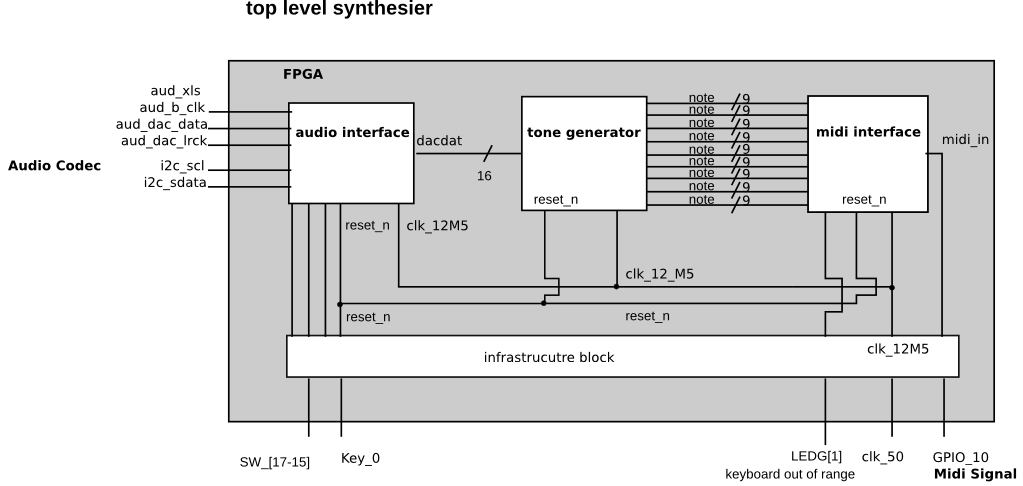
\includegraphics[width=1\textwidth]{images/midi_interface/top_synthesizer_block.png}
	\caption{Top Synthesizer mit MIDI Interface: Blockschaltbild}
	\label{fig.top_synthesizer_block}
\end{figure}

Hier ist das Konzept der Umsetzung des MIDI Interface detaillierter beschrieben:\\
\begin{figure}[H]
	\centering
	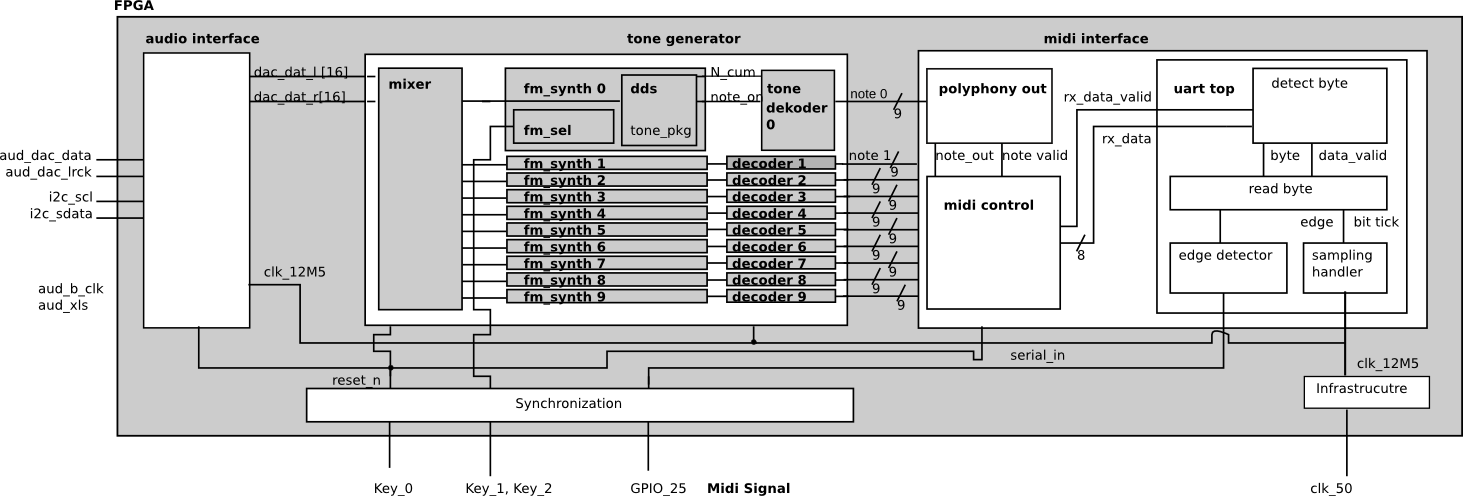
\includegraphics[width=1\textwidth]{images/midi_interface/top_synthesizer_detail.png}
	\caption{Top Synthesizer mit MIDI Interface: Detailansicht}
	\label{fig.top_synthesizer_detail}
\end{figure}




